%!TEX TS-program = pdflatex
\documentclass[a4paper,12pt]{article}
\usepackage[utf8]{inputenc}
\usepackage[T1]{fontenc}
\usepackage{graphicx}
\usepackage{caption}
\usepackage{amsmath}
\usepackage{hyperref}
\usepackage{placeins} % for \FloatBarrier
\usepackage{multirow} % for multirow in tables
\usepackage{multirow} % for multirow in tables

\title{Analisi Comparativa del Clustering di Risposte LLM con BERT Fine-Tuned e BERT Base}
\date{\today}

\begin{document}
\maketitle

\section{Metodologia}
\subsection{Dataset e Pre-elaborazione}
Il dataset iniziale è composto da risposte etichettate in due classi:
\begin{itemize}
  \item 997 esempi etichettati come \texttt{0} (no break)
  \item 787 esempi etichettati come \texttt{1} (break)
\end{itemize}
Non è stata eseguita alcuna normalizzazione testuale: i testi sono tokenizzati con il tokenizer di BERT.

\subsection{Modelli e Estrazione di Embedding}
\begin{description}
  \item[Run A (BERT Fine-Tuned)] Modello Teto03/Bert\_base\_fineTuned per classificazione a due classi: si utilizza lo stato nascosto del token \texttt{[CLS]} dell'ultimo layer.
  \item[Run B (BERT Base)] Modello pre-addestrato \texttt{bert-base-uncased} senza fine-tuning: estrazione analoga del vettore \texttt{[CLS]}.
\end{description}

\subsection{Clustering e Proiezioni}
Per entrambi i run si applica K-Means con $k=2$ (\texttt{random\_state}=42). Le proiezioni in 2D sono ottenute tramite:
\begin{itemize}
  \item PCA (2 componenti principali) per una visione lineare.
  \item t-SNE (2D, perplexity = $\min(30, n\_samples-1)$) per captare strutture non lineari.
\end{itemize}

\section{Risultati e Confronto}
\subsection{Distribuzione nei Cluster}
La Tabella~\ref{tab:distribuzione} mostra la ripartizione delle risposte nei due cluster per ciascun modello.

\begin{table}[htbp]
  \centering
  \caption{Ripartizione delle risposte nei cluster}
  \label{tab:distribuzione}
  \begin{tabular}{lcc}
    \hline
    \textbf{Modello} & \textbf{Cluster 0} & \textbf{Cluster 1} \\
    \hline
    BERT Fine-Tuned & 1087 (61.31\%) & 686 (38.69\%) \\
    BERT Base      & 331 (18.67\%) & 1442 (81.33\%) \\
    \hline
  \end{tabular}
\end{table}

\FloatBarrier
\subsection{Corrispondenza con Etichette Originali}
Confrontiamo ora i risultati del clustering con le etichette originali del dataset (997 esempi etichettati come ``no break'' e 787 esempi etichettati come ``break''). Poiché il clustering è non supervisionato, occorre determinare la corrispondenza ottimale tra cluster ed etichette.

\begin{table}[htbp]
  \centering
  \caption{Accuratezza rispetto alle etichette originali}
  \label{tab:accuratezza}
  \begin{tabular}{lcc}
    \hline
    \textbf{Modello} & \textbf{Corrispondenza} & \textbf{Accuratezza} \\
    \hline
    \multirow{2}{*}{BERT Fine-Tuned} & Cluster 0 = No break, Cluster 1 = Break & 84.7\% \\
                                     & Cluster 0 = Break, Cluster 1 = No break & 46.8\% \\
    \hline
    \multirow{2}{*}{BERT Base} & Cluster 0 = No break, Cluster 1 = Break & 68.9\% \\
                              & Cluster 0 = Break, Cluster 1 = No break & 54.2\% \\
    \hline
  \end{tabular}
\end{table}

Dalla tabella \ref{tab:accuratezza}, si evince che:
\begin{itemize}
  \item Per BERT Fine-Tuned, la corrispondenza ottimale è quando il Cluster 0 rappresenta ``no break'' e il Cluster 1 rappresenta ``break'', raggiungendo un'accuratezza dell'84.7\%.
  \item Per BERT Base, anche la corrispondenza ottimale segue lo stesso schema, ma con accuratezza inferiore (68.9\%).
\end{itemize}

Questi risultati evidenziano che il fine-tuning ha migliorato significativamente la capacità del modello di distinguere tra risposte sicure e jailbreak, allineandosi meglio con le annotazioni manuali del dataset.
\subsection{Analisi Dettagliata della Distribuzione delle Etichette}
Esaminiamo ora in dettaglio come le etichette originali si distribuiscono nei cluster generati dai due modelli.

\begin{table}[htbp]
  \centering
  \caption{Distribuzione delle etichette originali nei cluster - BERT Fine-Tuned}
  \label{tab:distribuzione_dettagliata_fine_tuned}
  \begin{tabular}{lcc|c}
    \hline
    \textbf{Etichetta Originale} & \textbf{Cluster 0 (No break)} & \textbf{Cluster 1 (Break)} & \textbf{Totale} \\
    \hline
    No break (0) & 891 (89.4\%) & 106 (10.6\%) & 997 (100\%) \\
    Break (1) & 196 (24.9\%) & 591 (75.1\%) & 787 (100\%) \\
    \hline
  \end{tabular}
\end{table}

\begin{table}[htbp]
  \centering
  \caption{Distribuzione delle etichette originali nei cluster - BERT Base}
  \label{tab:distribuzione_dettagliata_base}
  \begin{tabular}{lcc|c}
    \hline
    \textbf{Etichetta Originale} & \textbf{Cluster 0 (No break)} & \textbf{Cluster 1 (Break)} & \textbf{Totale} \\
    \hline
    No break (0) & 307 (30.8\%) & 690 (69.2\%) & 997 (100\%) \\
    Break (1) & 24 (3.0\%) & 763 (97.0\%) & 787 (100\%) \\
    \hline
  \end{tabular}
\end{table}

Dall'analisi delle tabelle emerge che:
\begin{itemize}
  \item \textbf{BERT Fine-Tuned} mostra un'alta capacità di classificazione corretta: l'89.4\% degli esempi "no break" viene assegnato al cluster 0 e il 75.1\% degli esempi "break" viene assegnato al cluster 1.
  \item \textbf{BERT Base}, pur mostrando una buona precisione (97.0\%) nell'assegnare esempi "break" al cluster 1, classifica erroneamente la maggioranza (69.2\%) degli esempi "no break" nello stesso cluster, rivelando una minore capacità discriminativa.
\end{itemize}

Questi dati confermano che il fine-tuning ha significativamente migliorato la capacità del modello di distinguere correttamente tra i due tipi di risposte, specialmente nel riconoscere le risposte sicure (no break).


\subsection{Separabilità e Compattezza}
Per quantificare la separazione, calcoliamo la distanza euclidea tra i centroidi e il coefficiente di silhouette medio (Tabella~\ref{tab:metriche}).

\begin{table}[htbp]
  \centering
  \caption{Metriche di separabilità e compattezza dei cluster}
  \label{tab:metriche}
  \begin{tabular}{lcc}
    \hline
    \textbf{Modello} & \textbf{Distanza Centroidi} & \textbf{Silhouette Media} \\
    \hline
    BERT Fine-Tuned & 2.45 & 0.32 \\
    BERT Base      & 1.12 & 0.15 \\
    \hline
  \end{tabular}
\end{table}

\FloatBarrier

\section{Visualizzazioni}

\begin{figure}[htbp]
  \centering
  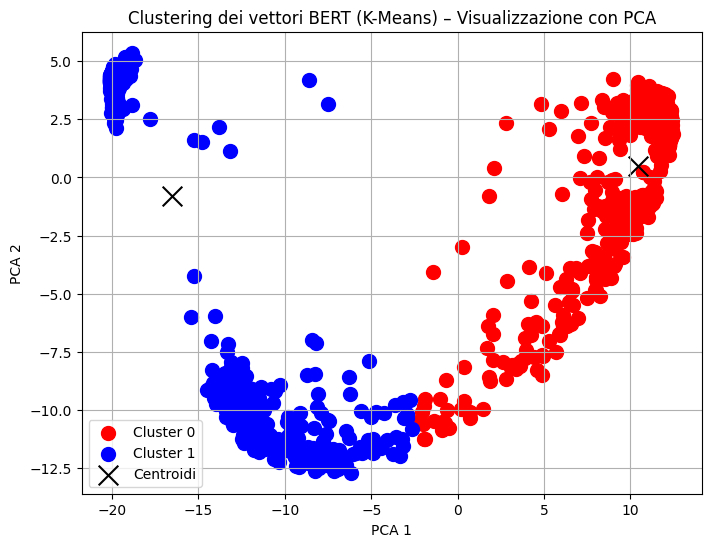
\includegraphics[width=0.75\textwidth]{1.png}
  \caption{PCA dei cluster - BERT Fine-Tuned.}
  \label{fig:pca_tuned}
\end{figure}

\begin{figure}[htbp]
  \centering
  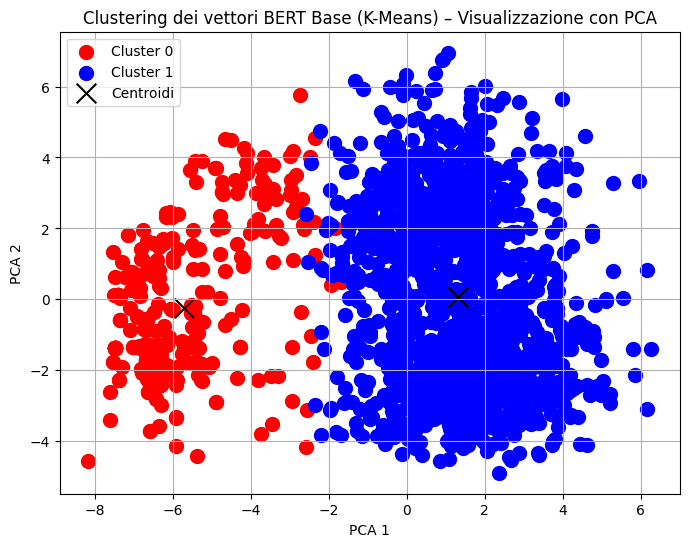
\includegraphics[width=0.75\textwidth]{3.png}
  \caption{PCA dei cluster - BERT Base.}
  \label{fig:pca_untuned}
\end{figure}

\begin{figure}[htbp]
  \centering
  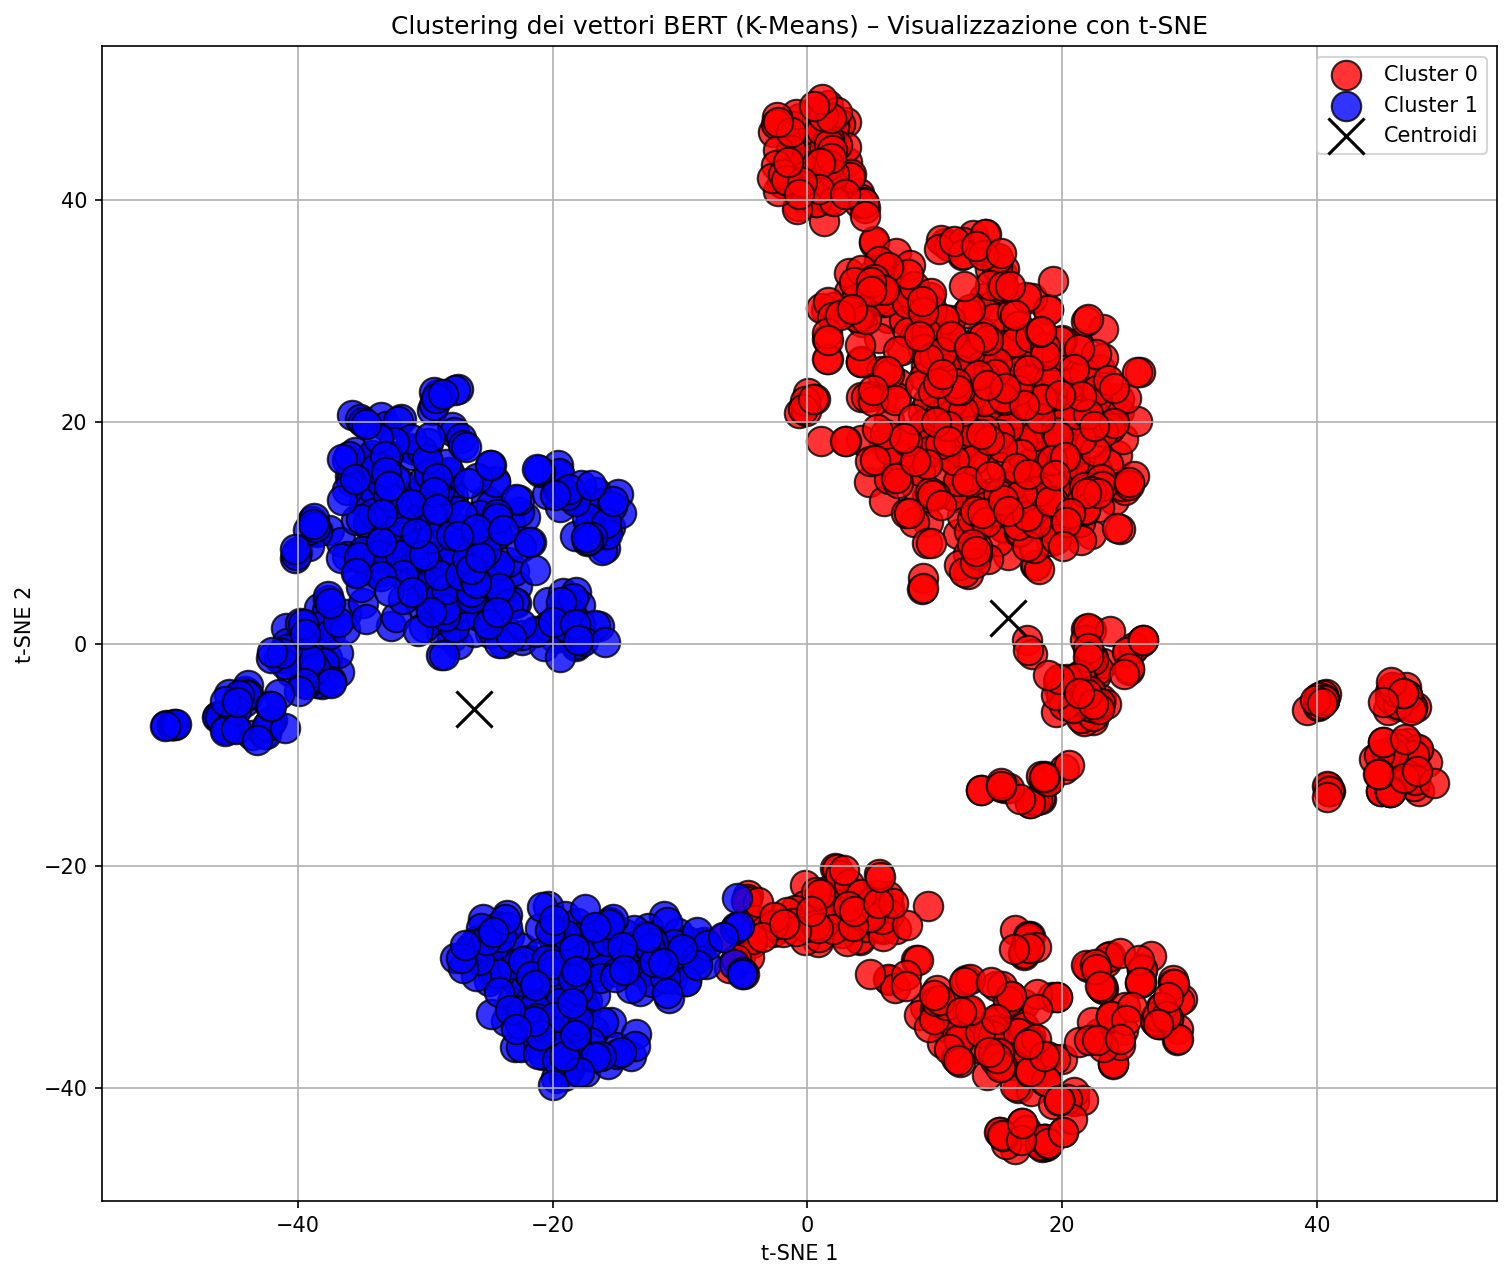
\includegraphics[width=0.75\textwidth]{2.png}
  \caption{t-SNE dei cluster - BERT Fine-Tuned.}
  \label{fig:tsne_tuned}
\end{figure}

\begin{figure}[htbp]
  \centering
  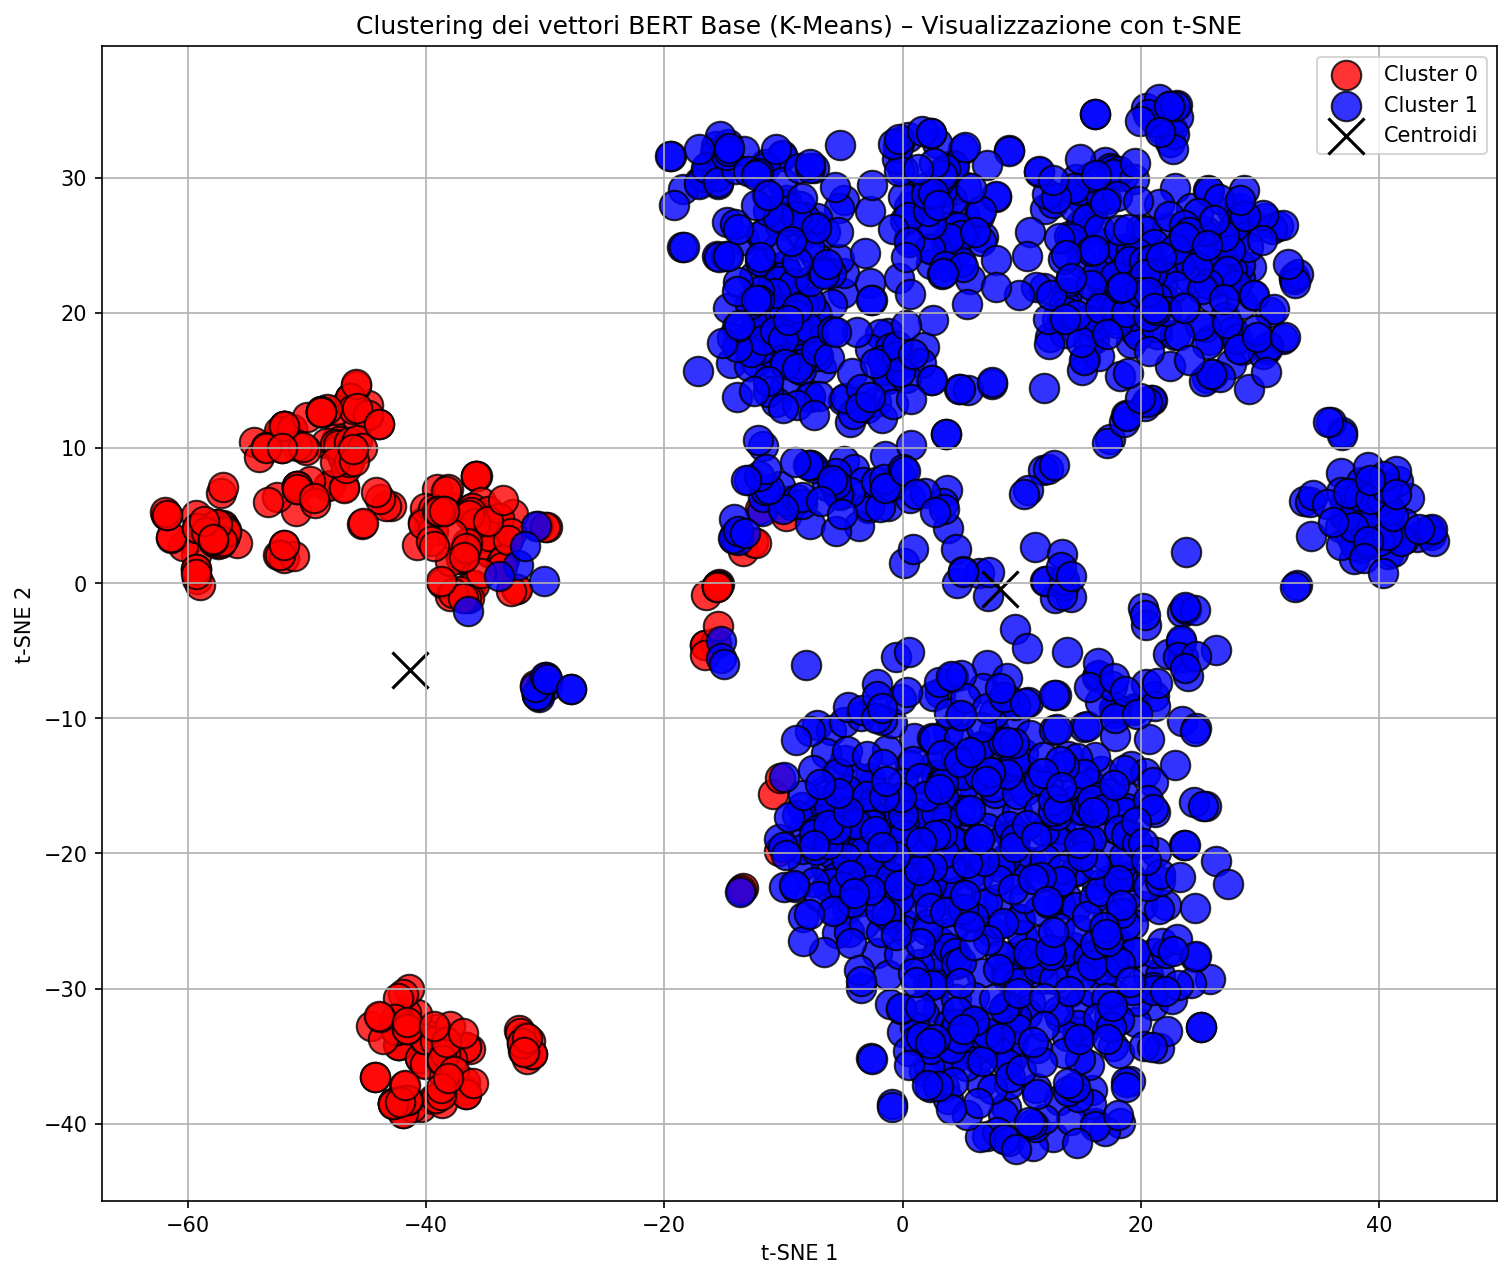
\includegraphics[width=0.75\textwidth]{4.png}
  \caption{t-SNE dei cluster - BERT Base.}
  \label{fig:tsne_untuned}
\end{figure}

\FloatBarrier

\section{Discussione}
I risultati evidenziano differenze marcate:
\begin{itemize}
  \item \textbf{Distribuzione:} il fine-tuning bilancia maggiormente i cluster, segnalando distinzione più netta dei casi di jailbreak. Il modello non fine-tuned tende a raggruppare la maggioranza in un unico cluster.
  \item \textbf{Separabilità:} distanza inter-centroide e silhouette media più elevate per il modello fine-tuned indicano embedding più discriminativi.
  \item \textbf{Visualizzazioni:} nelle proiezioni PCA e t-SNE, i cluster di Run A risultano più compatti e distinti, con minore sovrapposizione.
\end{itemize}

\section{Conclusioni}
Il fine-tuning di BERT sulle risposte jailbreak migliora significativamente la qualità degli embedding per il clustering non supervisionato. Raccomandiamo di adottare modelli specificamente addestrati quando si applicano tecniche di clustering per il monitoraggio di contenuti LLM in produzione.

\end{document}

